%!TEX TS-program = xelatex

% Шаблон документа LaTeX создан в 2018 году
% Алексеем Подчезерцевым
% В качестве исходных использованы шаблоны
% 	Данилом Фёдоровых (danil@fedorovykh.ru) 
%		https://www.writelatex.com/coursera/latex/5.2.2
%	LaTeX-шаблон для русской кандидатской диссертации и её автореферата.
%		https://github.com/AndreyAkinshin/Russian-Phd-LaTeX-Dissertation-Template

\documentclass[a4paper,14pt]{article}


%%% Работа с русским языком
\usepackage[english,russian]{babel}   %% загружает пакет многоязыковой вёрстки
\usepackage{fontspec}      %% подготавливает загрузку шрифтов Open Type, True Type и др.
\defaultfontfeatures{Ligatures={TeX},Renderer=Basic}  %% свойства шрифтов по умолчанию
\setmainfont[Ligatures={TeX,Historic}]{Times New Roman} %% задаёт основной шрифт документа
\setsansfont{Comic Sans MS}                    %% задаёт шрифт без засечек
\setmonofont{Courier New}
\usepackage{indentfirst}
\frenchspacing

\renewcommand{\epsilon}{\ensuremath{\varepsilon}}
\renewcommand{\phi}{\ensuremath{\varphi}}
\renewcommand{\kappa}{\ensuremath{\varkappa}}
\renewcommand{\le}{\ensuremath{\leqslant}}
\renewcommand{\leq}{\ensuremath{\leqslant}}
\renewcommand{\ge}{\ensuremath{\geqslant}}
\renewcommand{\geq}{\ensuremath{\geqslant}}
\renewcommand{\emptyset}{\varnothing}

%%% Дополнительная работа с математикой
\usepackage{amsmath,amsfonts,amssymb,amsthm,mathtools} % AMS
\usepackage{icomma} % "Умная" запятая: $0,2$ --- число, $0, 2$ --- перечисление

%% Номера формул
%\mathtoolsset{showonlyrefs=true} % Показывать номера только у тех формул, на которые есть \eqref{} в тексте.
%\usepackage{leqno} % Нумерация формул слева	

%% Перенос знаков в формулах (по Львовскому)
\newcommand*{\hm}[1]{#1\nobreak\discretionary{}
	{\hbox{$\mathsurround=0pt #1$}}{}}

%%% Работа с картинками
\usepackage{graphicx}  % Для вставки рисунков
\graphicspath{{images/}}  % папки с картинками
\setlength\fboxsep{3pt} % Отступ рамки \fbox{} от рисунка
\setlength\fboxrule{1pt} % Толщина линий рамки \fbox{}
\usepackage{wrapfig} % Обтекание рисунков текстом

%%% Работа с таблицами
\usepackage{array,tabularx,tabulary,booktabs} % Дополнительная работа с таблицами
\usepackage{longtable}  % Длинные таблицы
\usepackage{multirow} % Слияние строк в таблице
\usepackage{float}% http://ctan.org/pkg/float

%%% Программирование
\usepackage{etoolbox} % логические операторы


%%% Страница
\usepackage{extsizes} % Возможность сделать 14-й шрифт
\usepackage{geometry} % Простой способ задавать поля
\geometry{top=20mm}
\geometry{bottom=20mm}
\geometry{left=20mm}
\geometry{right=10mm}
%
%\usepackage{fancyhdr} % Колонтитулы
% 	\pagestyle{fancy}
%\renewcommand{\headrulewidth}{0pt}  % Толщина линейки, отчеркивающей верхний колонтитул
% 	\lfoot{Нижний левый}
% 	\rfoot{Нижний правый}
% 	\rhead{Верхний правый}
% 	\chead{Верхний в центре}
% 	\lhead{Верхний левый}
%	\cfoot{Нижний в центре} % По умолчанию здесь номер страницы

\usepackage{setspace} % Интерлиньяж
\onehalfspacing % Интерлиньяж 1.5
%\doublespacing % Интерлиньяж 2
%\singlespacing % Интерлиньяж 1

\usepackage{lastpage} % Узнать, сколько всего страниц в документе.

\usepackage{soul} % Модификаторы начертания

\usepackage{hyperref}
\usepackage[usenames,dvipsnames,svgnames,table,rgb]{xcolor}
\hypersetup{				% Гиперссылки
	unicode=true,           % русские буквы в раздела PDF
	pdftitle={Разработка программной системы для автоматической генерации графа диалогов по текстам пьес.},   % Заголовок
	pdfauthor={Подчезерцев А.Е.},      % Автор
	pdfsubject={ВКР},      % Тема
	pdfcreator={Подчезерцев А.Е.}, % Создатель
	pdfproducer={Подчезерцев А.Е.}, % Производитель
	pdfkeywords={keyword1} {key2} {key3}, % Ключевые слова
	colorlinks=true,       	% false: ссылки в рамках; true: цветные ссылки
	linkcolor=black,          % внутренние ссылки
	citecolor=black,        % на библиографию
	filecolor=magenta,      % на файлы
	urlcolor=black           % на URL
}
\makeatletter 
\def\@biblabel#1{#1. } 
\makeatother
\usepackage{cite} % Работа с библиографией
%\usepackage[superscript]{cite} % Ссылки в верхних индексах
%\usepackage[nocompress]{cite} % 
\usepackage{csquotes} % Еще инструменты для ссылок

\usepackage{multicol} % Несколько колонок

\usepackage{tikz} % Работа с графикой
\usepackage{pgfplots}
\usepackage{pgfplotstable}

\usepackage{ dsfont }

\newcommand{\imref}[1]{рис.~\ref{#1}}

\usepackage{spreadtab}
\newcolumntype{K}[1]{@{}>{\centering\arraybackslash}p{#1cm}@{}}


\usepackage{xparse}
\usepackage{fancyvrb}

\RecustomVerbatimCommand{\VerbatimInput}{VerbatimInput}
{
	fontsize=\footnotesize    
}

\newcolumntype{?}[1]{!{\vrule width #1}}

\usepackage{tocloft}
\renewcommand{\cftsecleader}{\cftdotfill{\cftdotsep}}

\usepackage{pdfpages}

\usepackage{rotating}

\usepackage{pdflscape}

\usepackage{ragged2e}
\usepackage{microtype}

% Выравнивание по ширине без переносов слов
\justifying
\sloppy
\tolerance=500
\hyphenpenalty=10000
\emergencystretch=3em

% Подогнать таблицу под ширину страницы
\usepackage{adjustbox}

\usepackage{titlesec}

% ГОСТ заголовки таблицы
\usepackage[font=small]{caption}

\captionsetup[figure]{justification=centering,labelsep=period} % Картинки по центру, с точкой после рис

\DeclareCaptionLabelFormat{rightline}{\rightline{\bothIfFirst{#1}{ }#2}}
\captionsetup[table]{justification=centering,labelformat=rightline,labelsep=newline}

\newcommand{\tablecaption}[1]{\addtocounter{table}{1}\small \begin{flushright}\tablename \ \thetable\end{flushright}%	
	\begin{center}#1\end{center}}

\usepackage{enumerate}
\begin{document} % конец преамбулы, начало документа
	%\begin{titlepage}
	\begin{center}
 		ФЕДЕРАЛЬНОЕ  ГОСУДАРСТВЕННОЕ АВТОНОМНОЕ \\
		ОБРАЗОВАТЕЛЬНОЕ УЧРЕЖДЕНИЕ ВЫСШЕГО ОБРАЗОВАНИЯ\\
		«НАЦИОНАЛЬНЫЙ ИССЛЕДОВАТЕЛЬСКИЙ УНИВЕРСИТЕТ\\
		«ВЫСШАЯ ШКОЛА ЭКОНОМИКИ»
	\end{center}
	
	\begin{center}
		\textbf{Московский институт электроники и математики}
		
		\textbf{им. А.Н.Тихонова НИУ ВШЭ}
		
		\vspace{2ex}
		
		\textbf{Департамент компьютерной инженерии}
	\end{center}
	\vspace{1ex}	
	
	\begin{center}
		Курс «Системное проектирование цифровых устройств»
	\end{center}	
	
	
	\begin{center}
	\textbf{ОТЧЕТ\\
		ПО ЛАБОРАТОРНОЙ РАБОТЕ №1
	}
	\end{center}	

	\begin{center}
		Тема работы: «Разработка и программирование Soft-процессорных ядер с архитектурой однотактный MIPS. Часть 1»
	\end{center}

	\vspace{2ex}

	\begin{flushright}
		\textbf{Выполнили:}
		
		\vspace{2ex}
		
		Студенты группы БИВ174
		
		Бригада №5
		
		\vspace{2ex}
		
		Подчезерцев Алексей Евгеньевич
		
		Солодянкин Андрей Александрович
		\vspace{2ex}
		
		\textbf{Принял:}
		
		асс. МИЭМ НИУ ВШЭ
		
		Американов А.А.
		
	\end{flushright}

	\vfill
	\begin{center}
		Москва \the\year \, г.
	\end{center}
	
\end{titlepage}
\addtocounter{page}{1}
	%\tableofcontents
	%\pagebreak
	
	\section{}
	Солодянкин Андрей;
	
	БИВ174;
	
	Исследование афинных преобразований в семантическом пространстве BERT.
	%\pagebreak
	
	\section{Актуальность}
	%2-3 страницы.
	
	%В последние годы компьютеры стали незаменимой частью нашей жизни, они представлены голосовыми помощниками, рекомендательными системами, системами умных домов, умными машинами и другими устройствами.
	%Важной частью всех этих систем являются модули, которые позволяют донести до компьютера 
	
	В последние годы технологии машинного обучения стали неотъемлемой частью нашей жизни.
	Они представлены голосовыми помощниками, рекомендательными системами, умными домами, умными автомобилями и другими системами.
	Важной частью этих систем являются модули, которые помогают сделать понятным для компьютера то, что от него требуется.
	Для систем по обработке текста это модули обработки естественного языка или Natural Language Processing (NLP).
	
	Направление обработки естественного языка активно развивается, последний большой прорыв был сделан в 2018 году командой Google AI. 
	Была представлена новая модель обработки естественного языка под названием BERT или Bidirectional Encoder Representations from Transformers \cite{bert}. 
	BERT продемонстрировал лучшее качество на тесте SQuAD (Stanford Question Answering Dataset) \cite{SQuAD} версии 1.1 для вопросно-ответных систем. На рисунке \ref{fig:quality_bert} представлены первые строчки таблицы лидеров для теста SQuAD 1.1 на момент выхода модели BERT.
	
	\begin{figure}[H]
		\centering
		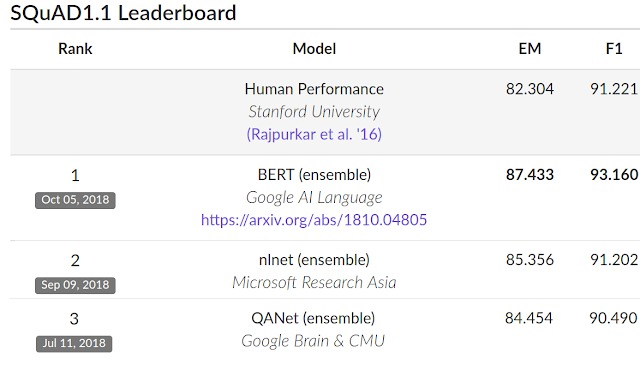
\includegraphics[width=0.6\linewidth]{images/2018-11-03.-bert-nlp-method_2}
		\caption{Сравнение BERT с другими моделями на момент выхода модели}
		\label{fig:quality_bert}
	\end{figure}
	
	Сейчас появились модели с качеством лучше, чем у модели BERT. 
	При этом многие модели с хорошим качеством на второй версии теста SQuAD \cite{SQuAD} (SQuAD 2.0 \cite{SQuAD2}) используют те же принципы, что и модель BERT.
	На рисунке \ref{fig:quality140321} представлен топ 3 моделей на тесте SQuAD 2.0 \cite{SQuAD2} от 14.03.21.
	
	\begin{figure}[H]
		\centering
		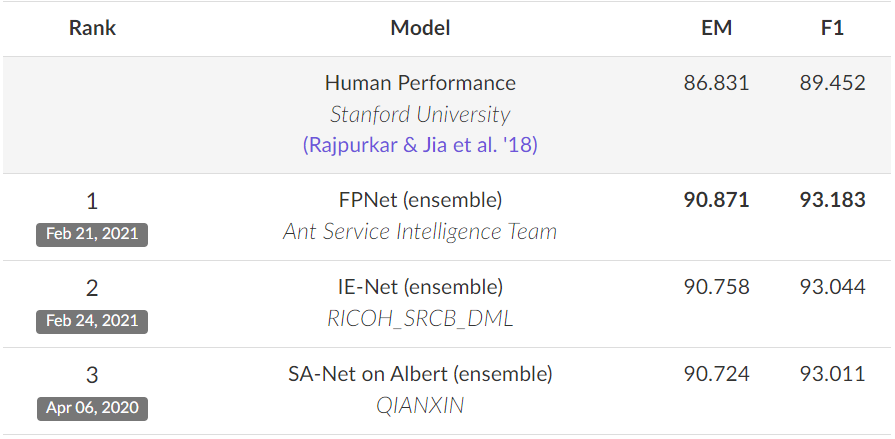
\includegraphics[width=0.6\linewidth]{images/quality_14_03_21}
		\caption{Таблица лидеров теста SQuAD2.0 на 14.03.21}
		\label{fig:quality140321}
	\end{figure}

	При всей популярности модели BERT остаются аспекты которые, плохо изучены или вообще не изучены, например, влияние вложений друг на друга в одном предложении.
	Большинство людей работают с моделью, не понимая, что происходит в модели и как модель генерирует результаты.
	Происходит это из-за того, что трудно интерпретировать промежуточные данные.
	Кроме того, в промышленной сфере есть потребность в интерпретации моделей машинного обучения.
	
	Появляется потребность в интерпретации промежуточных данных.
	Промежуточными данными BERT являются эмбеддинги.
	Идея эмбеддингов заключается в том, что каждому слову ставится в соответствие вещественный многомерный вектор, что позволяет не просто представить текст в численном виде для работы компьютера с ним, но также применять векторные операции, выражая с их помощью различные семантические отношения между словами. 
	В нашей работе проверяется гипотеза о возможности аффинных преобразований для эмбедднгов слов в семантическом пространстве BERT и проводится оценка качества проведенных аффинных преобразований.
	Это позволит приблизиться к пониманию эмбеддингов слов в модели BERT.
	

	
	
	

	\pagebreak
	
	\section{Обзор литературы}
	%минимум 30 работ
	%10-15 страниц
	
	Для того, чтобы исследовать аффинные преобразования в семантическом пространстве BERT необходимо понимать истоию развития NLP, как работают аффинные преобразования в других моделях NLP, как устроена модель BERT и какие исследования и эксперименты уже проведены с моделью BERT.
	
	\subsection{История развития}
	
	Обработка естественного языка берет свое начало в 1950-х годах. Уже в 1950 году Алан Тьюринг опубликовал статью под названием «Вычислительные машины и интеллект », в которой предлагалось то, что сейчас называется тестом Тьюринга в качестве критерия интеллекта, задача, которая включает автоматическую интерпретацию и создание естественного языка, но в то время не сформулирована как проблема, отдельная от искусственного интеллекта.
	
	%https://wikichi.ru/wiki/Natural_language_processing
	
	\subsection{Обзор других моделей}
	
	
	
	\subsection{Устройство модели BERT}
	
	Устройство модели описано в [\today].  
	
	\subsection{Исследования и эксперименты BERT}
	
	\subsection{Выводы}

	\pagebreak
	
	\section{Постановка задачи}
	%0.5-1 страница
	%задачи (минимум 8)

	\pagebreak
	
	
	
	
	
	\newpage 
	\renewcommand{\refname}{{\normalsize Список использованных источников}} 
	\centering 
	
	%\bibliographystyle{gost780s} % ГОСТ 7.80
	%\bibliography{biblio} % MachLearn.bib
	
	\begin{thebibliography}{9} 
		\addcontentsline{toc}{section}{\refname} 
		\bibitem{bert}Devlin J. et al. Bert: Pre-training of deep bidirectional transformers for language understanding //arXiv preprint
		\bibitem{SQuAD}Rajpurkar P. et al. Squad: 100,000+ questions for machine comprehension of text //arXiv preprint arXiv:1606.05250. – 2016.
		\bibitem{SQuAD2}Rajpurkar P., Jia R., Liang P. Know what you don't know: Unanswerable questions for SQuAD //arXiv preprint arXiv:1806.03822. – 2018.
		\bibitem{turing}Turing A. M. Intelligent machinery. – 1948.
		
		
	\end{thebibliography}
	
\end{document} % конец документа
